% \documentclass[linenumbers,floatfix,ApJL,twocolumn]{aastex631}
\documentclass[floatfix,ApJL,twocolumn]{aastex631}

\usepackage{amssymb}
\usepackage{amsmath}
\usepackage{microtype}
\usepackage{url}
\usepackage{xspace}
\usepackage{xcolor}
\usepackage{ifxetex}
\ifxetex
\usepackage{fontspec}
\defaultfontfeatures{Extension = .otf}
\fi
\usepackage{fontawesome5}

\setlength{\parindent}{3.0ex}


% Projects:
\newcommand{\project}[1]{\textsf{#1}}

\newcommand{\python}{\project{Python}}
\newcommand{\cython}{\project{Cython}}
\newcommand{\cpp}{\project{C++}}
\newcommand{\jupyter}{\project{Jupyter}}

\newcommand{\exoplanet}{\project{exoplanet}}
\newcommand{\lightkurve}{\project{lightkurve}}
\newcommand{\starry}{\project{starry}}
\newcommand{\theano}{\project{Theano}}
\newcommand{\pymc}{\project{PyMC3}}
\newcommand{\celerite}{\project{celerite}}
\newcommand{\dynesty}{\project{dynesty}}
\newcommand{\astroquery}{\project{astroquery}}
\newcommand{\scipy}{\project{scipy}}
\newcommand{\jupytext}{\project{jupytext}}
\newcommand{\sphinx}{\project{sphinx}}
\newcommand{\jupyterbook}{\project{Jupyter-book}}
\newcommand{\arviz}{\project{ArviZ}}
\newcommand{\nbconvert}{\project{nbconvert}}


\newcommand{\tess}{\project{TESS}}
\newcommand{\kepler}{\project{Kepler}}
\newcommand{\gaia}{\project{Gaia}}

\newcommand{\mast}{\project{MAST}}
\newcommand{\exofop}{\project{ExoFOP}}

\newcommand{\tessAtlas}{\project{TESS Atlas}}

% math
\newcommand{\T}{\ensuremath{\mathrm{T}}}
\newcommand{\dd}{\ensuremath{ \mathrm{d}}}
\newcommand{\unit}[1]{{\ensuremath{ \mathrm{#1}}}}
\newcommand{\bvec}[1]{{\ensuremath{\boldsymbol{#1}}}}


\DeclareMathOperator{\invG}{Inv-\mathnormal{\Gamma}}
\DeclareMathOperator{\N}{\mathcal{N}}
\DeclareMathOperator{\U}{\mathcal{U}}
\DeclareMathOperator{\Un}{\mathcal{U}}
\DeclareMathOperator{\Par}{\mathcal{P}ar}
\DeclareMathOperator{\tmin}{\mathnormal{t_{\rm min}}}
\DeclareMathOperator{\tmax}{\mathnormal{t_{\rm max}}}





%% affiliation shortcuts
\newcommand{\SPA}{School of Physics and Astronomy, Monash University, Clayton VIC 3800, Australia}
\newcommand{\OzGravMonash}{OzGrav: The ARC Centre of Excellence for Gravitational Wave Discovery, Clayton VIC 3800, Australia}
\newcommand{\AMNH}{Department of Astrophysics, American Museum of Natural History, New York, NY 10024, USA}
\newcommand{\CCA}{Center for Computational Astrophysics, Flatiron Institute, New York, NY 10010, USA}
\newcommand{\CUNY}{Graduate Center, City University of New York, 365 5th Avenue, New York, NY 10016, USA}
\newcommand{\BMCC}{Department of Science, BMCC, City University of New York, New York, NY 10007, USA}








\newcommand{\atlasUrl}{\href{http://catalog.tess-atlas.cloud.edu.au/}{catalog.tess-atlas.cloud.edu.au}}


\newcommand{\toiTemplateLink}{\href{https://github.com/dfm/tess-atlas/blob/main/src/tess_atlas/notebook_templates/toi_template.py}{github.com/dfm/tess-atlas/.../toi\_template.py}}

\newcommand{\paperPlotsLink}{\github{https://github.com/dfm/tess-atlas/blob/main/paper/figures/make_plots.py}}
\newcommand{\exoplanetOptimization}{\github{https://github.com/exoplanet-dev/pymc3-ext##optimization}}
\newcommand{\exoplanetDocs}{\href{https://docs.exoplanet.codes}{https://docs.exoplanet.codes/}}


\newcommand{\red}{\textcolor{red}}


\newcommand{\textuit}[1]{\textit{\underline{#1}}}



%% Numbers
% https://exoplanetarchive.ipac.caltech.edu/docs/counts_detail.html
% https://exoplanetarchive.ipac.caltech.edu/index.html


\newcommand{\numConfirmedPlanets}{5,090} % 
\newcommand{\numCandidatesRemaining}{6,959}

\newcommand{\numTessCandidates}{5,488} % 
\newcommand{\numTessPlanets}{227}
\newcommand{\numAnalysed}{2,833}
\newcommand{\numAnalysedMulti}{151}
\newcommand{\numAnalysedSingle}{68}
\newcommand{\cpuHrs}{$\sim80,000\ \rm{Hrs}$}

%% links
\newcommand{\atlasUrl}{\url{http://catalog.tess-atlas.cloud.edu.au/}}





\shorttitle{The \tess\ Atlas}


\begin{document}

\title{The \tess\ Atlas: an open source living catalog of TESS transit fits}

\correspondingauthor{Daniel Foreman-Mackey}
\email{foreman.mackey@gmail.com}

\author[0000-0002-4146-1132{Avi Vajpeyi}
\affiliation{
    School of Physics and Astronomy,
    Monash University,
    Clayton VIC 3800,
    Australia
}
\affiliation{
OzGrav: The ARC Centre of Excellence for Gravitational Wave Discovery,
Clayton VIC 3800,
Australia
}

\author[0000-0002-9328-5652]{Daniel Foreman-Mackey}
\affiliation{
    Center for Computational Astrophysics,
    Flatiron Institute,
    162 5th Ave,
    New York, NY 10010
}







\begin{abstract}
% The Transiting Exoplanet Survey Satellite \tess\ has enabled the discovery of more than five-thousand exoplanet candidates, out of which only a few hundred have been confirmed.
% Exoplanet confirmation requires vetting of candidates by ruling out false positives and follow-up observations and analyses.
We present the \tess\ Atlas, a living catalog of candidate exoplanet parameter estimates, from two-minute cadence \tess\  data, to assist the vetting process and follow-up analyses.
This catalog contains posterior estimates for \red{\numAnalysed} \tess\ Objects of Interest, including \red{\numAnalysedMulti} multi-planet candidate systems and \red{\numAnalysedSingle} candidates having data for a single transit.
Our analysis utilises the No-U-Turns Markov chain Monte Carlo algorithm to sample the parameter space with a circular transit model implemented in \exoplanet.
\avi{The \tess\ Atlas estimates are different from the ExoFop}.
We provide posterior samples from our analyses and \jupyter notebooks to reproduce the analyses for each exoplanet candidate.
\end{abstract}

% info on sectors: https://heasarc.gsfc.nasa.gov/docs/tess/sector.html

\keywords{%
  methods: data analysis ---
  methods: statistical ---
  miscellaneous --- catalogs --- surveys
}


\section{Introduction} \label{sec:intro}

In March 2022, NASA's exoplanet archive~\citep{Akeson:2013:PASP}\footnote{\href{https://exoplanetarchive.ipac.caltech.edu/}{https://exoplanetarchive.ipac.caltech.edu/}} surpassed five thousand confirmed exoplanets, a milestone made possible by data from several observatories, including the Transiting Exoplanet Survey Satellite TESS~\citep{Ricker:2015:JATIS}.
The confirmed exoplanets exhibit a wide range of masses, compositions, and radii.
Some of these planets are also located within their planetary systems' habitable zone.
Furthermore, the population of these exoplanets has fuelled research into planetary system architecture, planetary formation and evolution, and updated exoplanet occurrence rates.
These analyses will be more informative with a bigger sample of exoplanets and more precise estimates of the planet's characteristics.
This list of ~5000 exoplanets may be dramatically increased once the 6000 exoplanets awaiting validation are processed, more than half of which are candidates detected in TESS data.
The majority of TESS exoplanet candidates were discovered using the photometric transit method.
Unfortunately, systematic effects (e.g. ) and non-planetary astrophysical sources (e.g. stellar granulation and eclipsing binaries) can mimic exoplanet transits.
Hence, to validate these candidates, it is necessary to eliminate false positives and, if possible, conduct additional observations. 

% Targets are assigned consecutive TOI IDs. Multi- planet systems are assigned suffixes (.01, .02, etc.) mir- roring the suffixes assigned for the TCE. TEV automat- ically generates a comma-separated values (CSV) file with all necessary parameters for each TOI from the vetted TOI list. Each TOI has a table of pa- rameters, a DV summary page, and a full DV report.


This motivates constructing a homogeneous method of \tess\ Atlas, a catalog of transiting exoplanet posterior estimates for the \red{\numAnalysed} \tess\ Objects of Interest (TOIs) with two-minute cadence observations from 2018 through 2022.
The catalog of posteriors, summary statistics, and software to reproduce the analyses are provided at \atlasUrl.
The website contains a \jupyter\ notebook for each TOI, documenting the end-to-end analysis of each TOI.
The notebooks contain software to download and clean light curve data, the transit model and priors for inference implementations, the \pymc sampling stage, and a posterior post-processing step.
The website also documents the method to download our Bayesian parameter inference posterior samples, load them and make various plots.


We provide software to reproduce the analyses and results at \atlasUrl.
The website contains one Jupyter notebook for each TOI, demonstrating the end-to-end analysis of a TOI.
The notebooks contain software to download and clean light curve data, implementations of the transit-model and priors for inference, the \pymc sampling stage, and a posterior post-processing step.
The website also documents the method to download our Bayesian parameter inference posterior samples, load them and make various plots.


The remainder of the paper is organised as follows: Section~\ref{sec:method} describes our transit light curve model and the Bayesian framework we use to estimate parameters of exoplanet systems from the observed data.
The analysis results are summarised in Section~\ref{sec:results}.
The catalog, released data, and software to reproduce the results are described in Section~\ref{sec:data} and are available online as supplementary materials (\atlasUrl).
Finally, we provide concluding remarks in Section~\ref{sec:conclusion}.

\section{Method} \label{sec:method}

In this section, we outline the procedures to analyse each TOI and generate the \tessAtlas. 


\subsection{Target selection and setup }

\begin{figure*}
    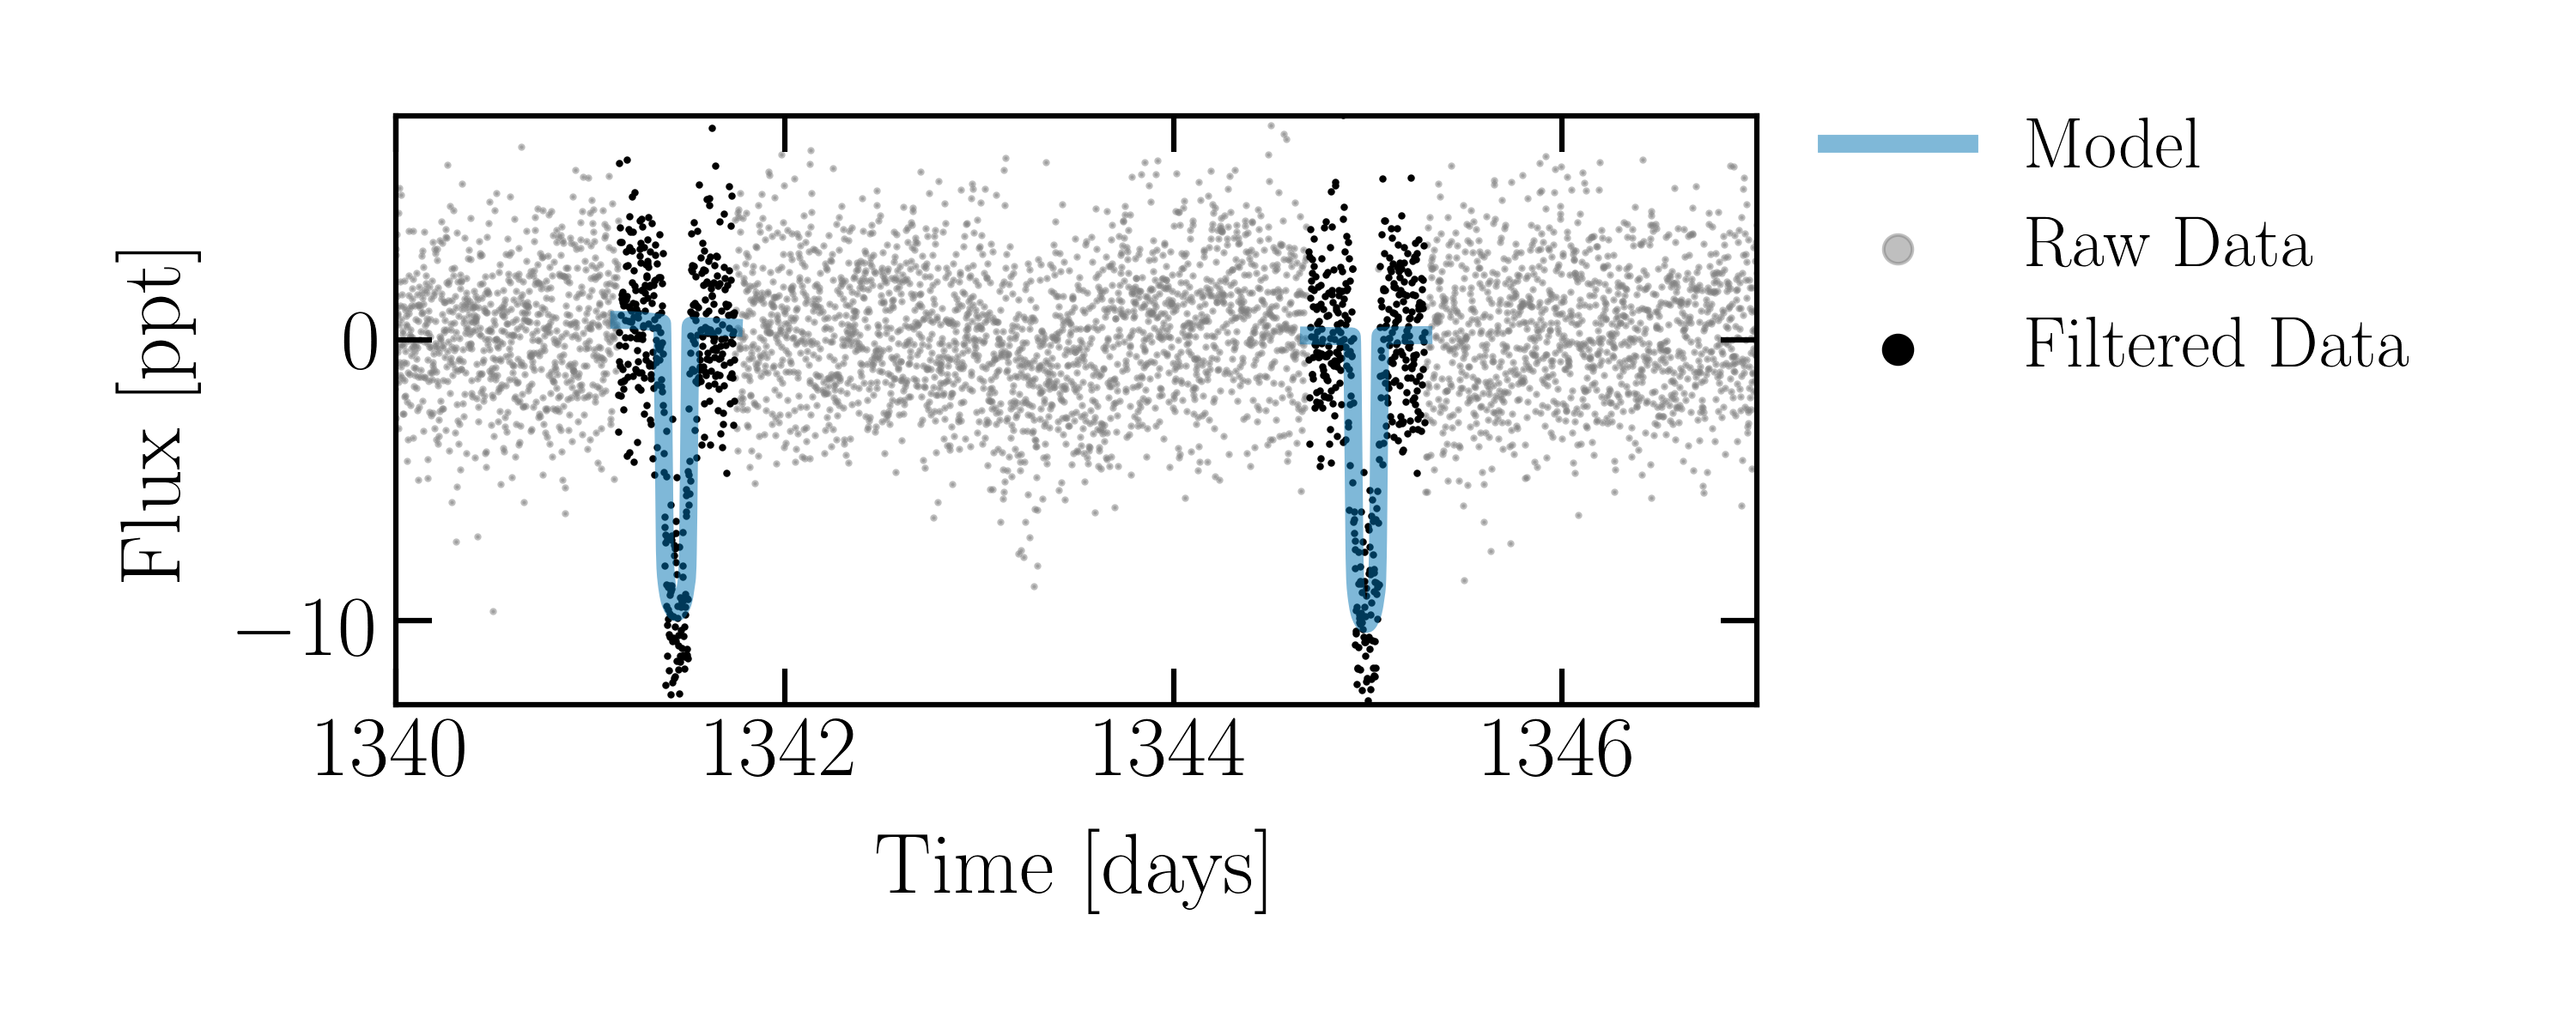
\includegraphics[width=\linewidth]{figures/raw_data_toi_103.png}
    \caption{\textbf{Light curve data for TOI-103 (from 1030-1450 BKJD):} The raw light curve data for TOI 103 is plotted in gray points, with \exofop\ best transit model parameter fit plotted on top in blue. The black points are obtained by filtering the raw data using the \exofop\ transit parameter estimates as described in the text. Code to reproduce this plot is on GitHub~\paperPlotsLink.}
    \label{fig:}
\end{figure*}

We obtain planetary parameters for \numTessCandidates TOIs with two-minute cadence data (as of Sept 2022) from the Exoplanet Follow-up Observing Program for TESS (\exofop) catalog.
This catalog reflects the best possible analysis when vetting the TOIs~\citep{Guerrero:2021:ApJS,}.
Any TOIs without a period measurement, or a period equal to zero, are flagged as single-transit systems. 
Using \lightkurve\ we download the TOI light curves generated by the TESS Science Processing Operations Center pipeline~\citep{Jenkins:2016:SPIE, Jenkins:2021:tsc2}, and stored in the Mikulski Archive for Space Telescopes (\mast).

As a pre-processing step, we filter out low-frequency outliers from the light curve by removing data points with a root-mean-square (RMS) value above five when subtracted to a \scipy’s Savitzky-Golay filter (with a window length of 11 and sigma of 100) version of the light curve. 
If the amount of data for a light curve is larger than $100,000$ datapoints an additional filtering step is applied. 
Assuming that the \exofop\ orbital period and phase are accurate, data outside the anticipated transit times (with a buffer of two times the expected transit duration) are discarded for large light curves.
A plot of {TOI 103}'s raw and filtered light curves, along with \exofop\'s transit model are displayed in Figure~\ref{fig:raw}.
Finally, if available, estimates for each TOIs host star's mass, radius and stellar density are downloaded from \mast. 



\subsection{Transit Model}

The host star's limb darkening profile is approximated using \citet{Kipping:2013:MNRAS}'s quadratic limb darkening law \citep{Claret:2000:A&A, Mandel:2002:ApJL}, parameterised in \starry~\citep{Luger:2019:AJ} by the baseline relative flux of the light curve $f_0$ and two quadratic limb-darkening parameters $u_1, u_2$.
The stellar variability (from e.g. asteroseismic oscillation of the star) is modelled with a \celerite~\citep{Foreman-Mackey:2017:ascl} Gaussian Process (GP), with a stochastically driven damped harmonic oscillator kernel in linear combination with a jitter term $J$, to capture misspecified error bars and model misspecification.
The GP requires three parameters: the quality factor $Q_{\rm GP}$, the undamped period of the oscillator $\rho_{\rm GP}$, and the standard deviation of the process $\sigma_{\rm GP}$. 
We model exoplanet transits as circular (non-interacting) Keplerian orbits around their host star, using \exoplanet~\citep{Foreman-Mackey:2021:JOSS}. 
Circular orbits permit the use of computationally efficient, analytical orbital dynamics calculations.
Additionally, circular orbits avoid degeneracies between eccentricity $e$, the argument of periastron $\omega$, impact parameter $b$, and planet radius $R_p$. 
Furthermore, the eccentricity can also be computed in post-processing, as described by \citet{Dawson:2012:ApJ}.
Each of the $n$ exoplanets in a system is parameterised by the planets'
\begin{itemize}
  \item \emph{two reference transit times}, one near the beginning of the observations, $\tmin[n]$, and one near the end, $\tmax[n]$, both measured in \tess\ BJD,
  \item \emph{the orbital period}, $P[n]$, measured in days,
  \item \emph{the number of periods}, $N_P[n]$, in the TESS observational baseline,
  \item \emph{the transit duration}, $\tau[n]$, measured in hours,
  \item \emph{the orbital impact parameter}, $b[n]$, constrained to be $|b| \le 1$,
  \item \emph{the approximate transit depth}, $\delta[n]$, measured in parts-per-thousand, and
  \item \emph{the radius ratio} $R_{\rm p}[n] / R_\star$, of the planet radius $R_{\rm p}[n]$ divided by the stellar radius $R_\star$.
\end{itemize}
Not all of the above parameters are required to model a transiting exoplanet. 
The choice of transiting exoplanet parameters utilised is discussed in the following section.

% Implementation details for the various model components are available on the \exoplanet\ documentation website\footnote{\exoplanetDocs}. 

\subsection{Inference Framework}

Uninformative priors are set for the stellar limb darkening (using the \citet{Kipping:2013:MNRAS} parameterisation), mean flux, and noise parameters.
The quality factor $Q_{\rm GP}$ prior is fixed to a delta function at zero point three.

The transiting exoplanet parameter priors are centred around \exofop\ estimates.
As transiting planet’s phase and period are tightly constrained, we enforce a delta prior to the number of periods $N_P[n]$ between the two references times $\tmin[n]$ and $\tmax[n]$.
The reference time priors are centred near the anticipated transit times and allowed a wide range of up to ten times the \exofop\ transit duration. 
The orbital period can later be calculated for each planet as 
\begin{equation}
  P[n] =  (\tmax[n] - \tmin[n]) / N_P[n]\, .
\end{equation}

If a planet only transits once in data recorded for a duration of time $t$, the prior on the second reference time $\tmax[n]$ is substituted with a prior on the planet's orbital period $P[n]$. 
As the orbital period for a single-transit planet is challenging to measure, a wide Pareto prior is placed on the period, with the minimum period $P_{\rm min}$ equal to
\begin{equation}
P_{\rm min}[n] = \rm{max} \left\{ \begin{array}{cl}
\tmin[n] - {\rm min}(t)\\
{\rm max}(t) - \tmin[n]
\end{array} \right. \, .
\end{equation} 
This prior provides more support for shorter periods.

Instead of setting a prior on the transit depth, we use the small planet approximation, 
\begin{equation}
    R_{\rm p}[n]/R_{\star} = \sqrt{\delta[n]}\, ,
\end{equation}
and set a log normal prior on radius ratio, centred at the \exofop\ radius ratio measurement.
The log normal radius ratio prior provides more support for systems with smaller ratios.
Finally, the impact parameter prior is uniform, conditioned on the radius ratio.
A full list of the priors is presented in Table~\ref{tab:priors}. 

\begin{table*}[]
\centering
\caption{\textbf{Priors table:} Table of priors on the light curve transit model parameters. We use shorthand to represent distributions: $\Un$~uniform (min, max), $\N$~normal ($\mu,\sigma$), $\Par$~Pareto ($\alpha$, min) and finally $\invG$~Inverse Gamma (lower, upper). The prime superscript (${}^{\prime}$) indicates values from \exofop.  Each planet in a $n$-planet system will have its unique planet priors. The $t_i$ parameter is shorthand for both $\tmin$ and $\tmax$. The $P$ prior is used only for planets with a single transit in data in place of $\tmax$. $P_{\rm min}$ is defined in the text. Finally, the prior on $b$ is conditional on $R_{\rm p}/R_{\star}$ (refer to \exoplanet\ documentation for details.)}\label{tab:priors}
\def\arraystretch{1.1} 
\setlength{\tabcolsep}{0.5em}
\begin{tabular}{cllcl}
\text{Parameter}      & \text{Distribution}  &  & \text{Parameter}    & \text{Distribution}                                                    \\ 
\cline{1-2} \cline{4-5} 
\text{Star}           &                      &  & \text{Planet[$n$]}  &                                                                        \\
$u_1, u_2$            & $\Un(0,1)$           &  & $R_{\rm p}/R_\star$ & $\ln \N(R_{\rm p}^{\prime}/R_\star, 1)$                                \\
$f_0$                 & $\N(0, 10)$          &  & $b$                 & $\Un(0, R_{\rm p}/R_\star +1)$                                         \\                            
\text{Noise}          &                      &  & $\tau/\rm{days}$    & $\ln\N(\ln\tau^{\prime}, 0.2) \in [4\, \rm{min},  10\tau^{\prime}]$    \\
$\rho_{\rm GP}$       & $\invG(0.5, 10)$     &  & $t_i/\rm{TBJD}$     & $\N(t_i^{\prime}, \tau^{\prime}) \in [t_i^{\prime}\pm10\tau^{\prime}]$ \\
$ \sigma_{\rm GP}, J$ & $\invG(1, 5)$        &  & $P/\rm{days}$       & $\Par(2/3, P_{\rm min})$                                               \\
$ Q_{\rm GP}$         & 0.3                  &  & $N_P$               & $N^{\prime}_P$                                       
\end{tabular}    
\end{table*}

We initialise the posterior sampler's at a high likelihood point, obtained by using \exoplanet's non-linear optimisation framework.
Following initial optimisation, the posterior distribution is sampled with \pymc's Hamiltonian Monte Carlo (HMC) No U-Turn Sampler~\citep{Betancourt:2017:arXiv, Hoffman:2011:arXiv,Salvatier:2016:ascl}.
The sampler is run on two chains for 4,000 steps with a burn-in of 2,000 steps.
We pass the chains to \arviz\ and compute the rank normalised $\hat{R}$ diagnostic statistic~\cite{Vehtari:2019:arXiv}.
Analyses with $\hat{R}>1.01$ are flagged to have convergence issues. 
Due to our model parameterization this often occurs for grazing transits when $b\sim1$~\cite{Gilbert:2022:AJ}.


\subsection{Eccentricity post processing}

For successful analyses, we conduct a post-processing step to compute the orbital eccentricity, $e$, and argument of periapsis, $\omega$, for each transiting planet. 
First, we use our measurements of transit observables to compute the implied stellar density (under the assumption of circular orbits), $\rho_{\rm circ}$. 
The expression for $\rho_{\rm circ}$ is derived in Appendix~\ref{apdx:stellar_density}.
Note that $\rho_{\rm circ}$ is not the same as the actual stellar density, $\rho_{\star}$, and is unique for each planet in an $n$-planet system \citep[see, for example,][]{Dawson:2012:ApJ, Kipping:2012:MNRAS}.
Following \citet{Dawson:2012:ApJ}, we use $\rho_{\rm circ}$ with a cataloged value of $\rho_\star$ (obtained from \mast) to generate weights. 
These are used to re-weight uniformly drawn $e$ and $\omega$ to get weighted posterior samples. 

\subsection{Analysis execution and website generation}

The analysis steps for a TOI, from data retrieval to post-processing, are implemented in a `template' \jupyter notebook \footnote{\toiTemplateLink}.
After duplicating the template for each TOI, we insert the TOI number in the notebooks and execute them in parallel with \nbconvert. 
Once execution is complete, we use \jupyterbook, a package built upon \sphinx\ to convert the pre-processed notebooks into web-pages.
These pages are deployed to the \tessAtlas\ website~\footnote{\atlasUrl},  along with the \jupyter\ notebooks, the raw data (the light curve data and \exofop\ estimates) and the analysis outputs (the HMC chains and re-weighted posteriors). 


\begin{figure*}
    \gridline{
        \fig{figures/planet_3_posterior.png}{0.5\linewidth}{}
        \fig{figures/ecc_3_posterior.png}{0.25\linewidth}{}
    }
    \caption{\textbf{TOI 174.03 Posteriors:} (Left) posteriors for the radius ratio $R_{\rm p}/R_\star$, impact parameter $b$, orbital period $P$ and transit duration $\tau$. (Right) re-weighted posteriors for eccentricity $e$ and the argument of periastron $\omega$. 
    The shaded regions depict the 1,2,3-$\sigma$ contours and the dashed lines in the 1D histograms are the 90\% credible intervals. 
    The numbers reported on top the of 1D histograms are the median values of the posteriors with the 90\% CI uncertainty.
    The overplotted red line indicates the transit parameters stored on \exofop. 
    Source code for this plot is provided in GitHub~\paperPlotsLink.}
    \label{fig:posteriors}
\end{figure*}


\begin{figure}
    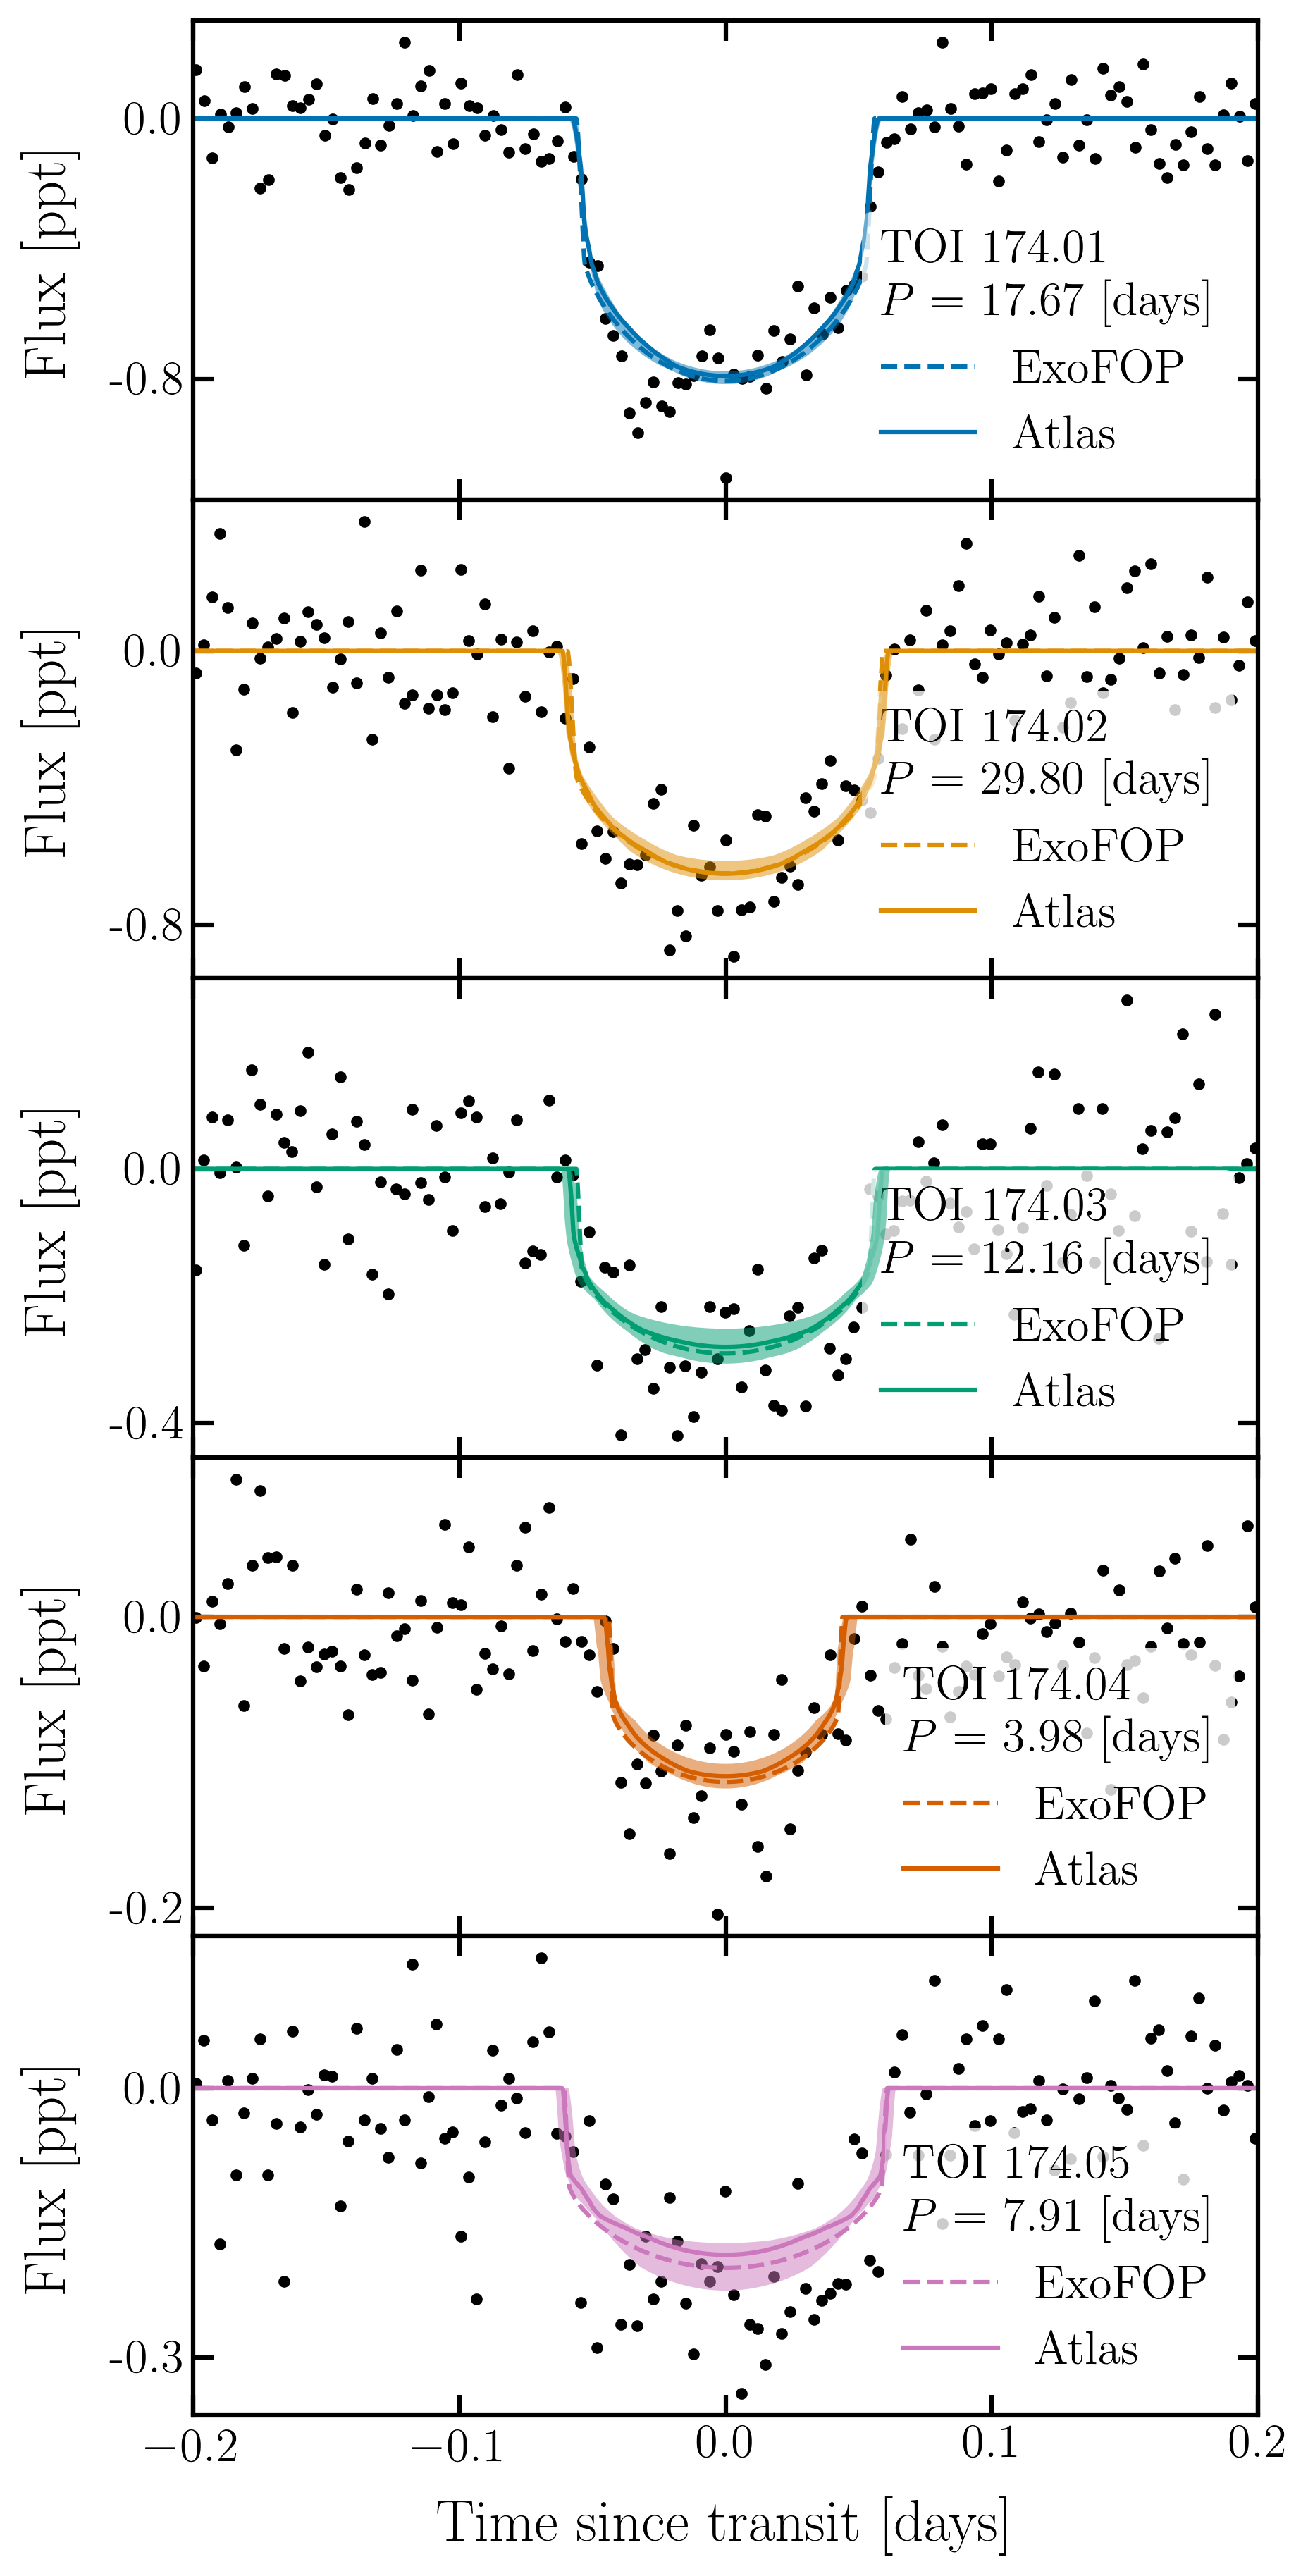
\includegraphics[width=0.9\linewidth]{paper/figures/toi_174_phase.png}
    \caption{\textbf{TOI 174 phase-folded light curve plots:} Each panel displays the phase-folded light curves of the five TOI 174.01-0.5 planets. 
    The light curve data points (black) have been binned to reduce visual clutter.
    The colorful shaded curves are the 
    }
    \label{fig:phase}
\end{figure}


These pages also include various plots at different stages of the analysis. 
For example, consider Figures~\ref{fig:corner}-\ref{fig:phase}.
These plots may help in future XX.


Finally, after the analysis for all TOIs complete, we also extract summary statistics, such as the median posterior parameters values and uncertainties on the parameters for all the TOIs. 
This is compied and also providedd on the TESS atlas website.






\section{Results}\label{sec:results}


We analysed XX TOIs. 
From these, YY analyses succeeded (the remaining analyses did not properly converge). 
The analysed systems contain XX systems with multiple planets, and XX planets with data for only a single transit. 




Our analysis of individual planets show posterior and phase plots match up. 
See the posterior and phase plots shoiw how the eofop analysos matchh.

Planet demographics: 
error for radius, explain plots.

Finally, show radius histogram, discuss radius valley, we display our
planet candidates in the planet radius–period space, and compare them with nearby candidates from the TOI and DIAmante catalogs, together with additional confirmed transiting planets observed in



\begin{figure}
  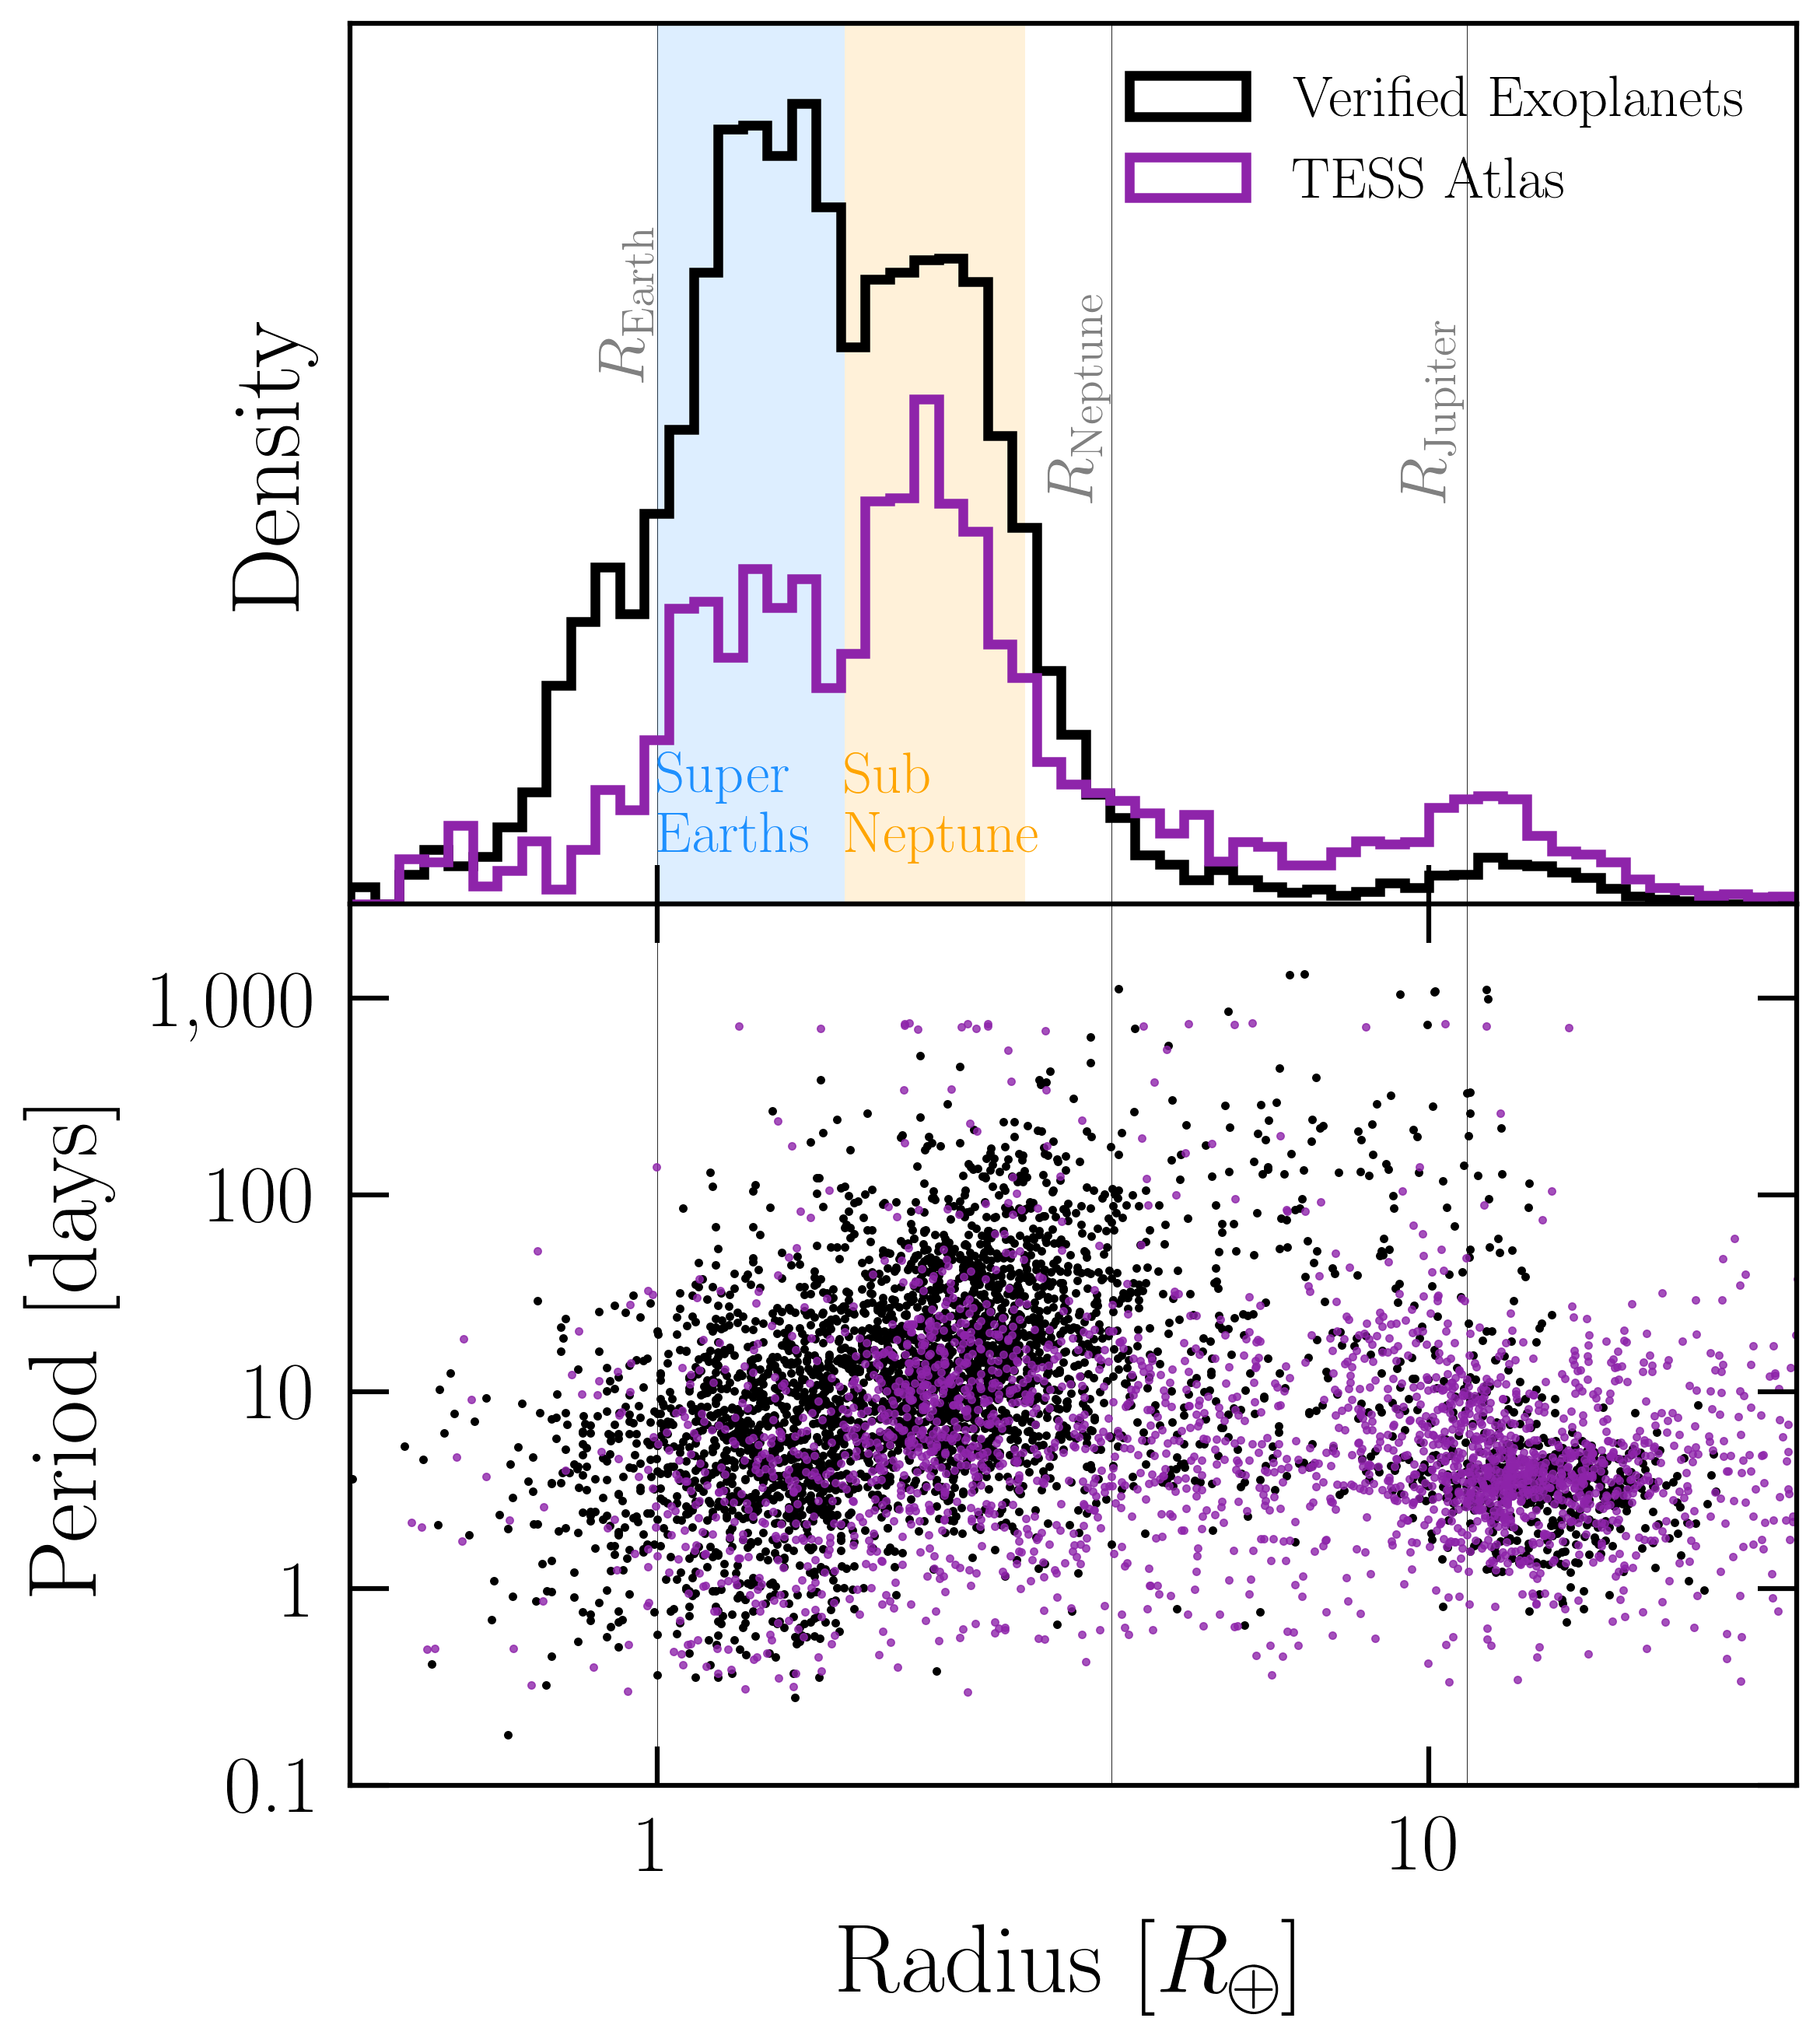
\includegraphics[width=\linewidth]{figures/radius_period_plot.png}
  \caption{\textbf{Exoplanet population radius distribution:} stuff }
  \label{fig:}
\end{figure}


\begin{figure}
  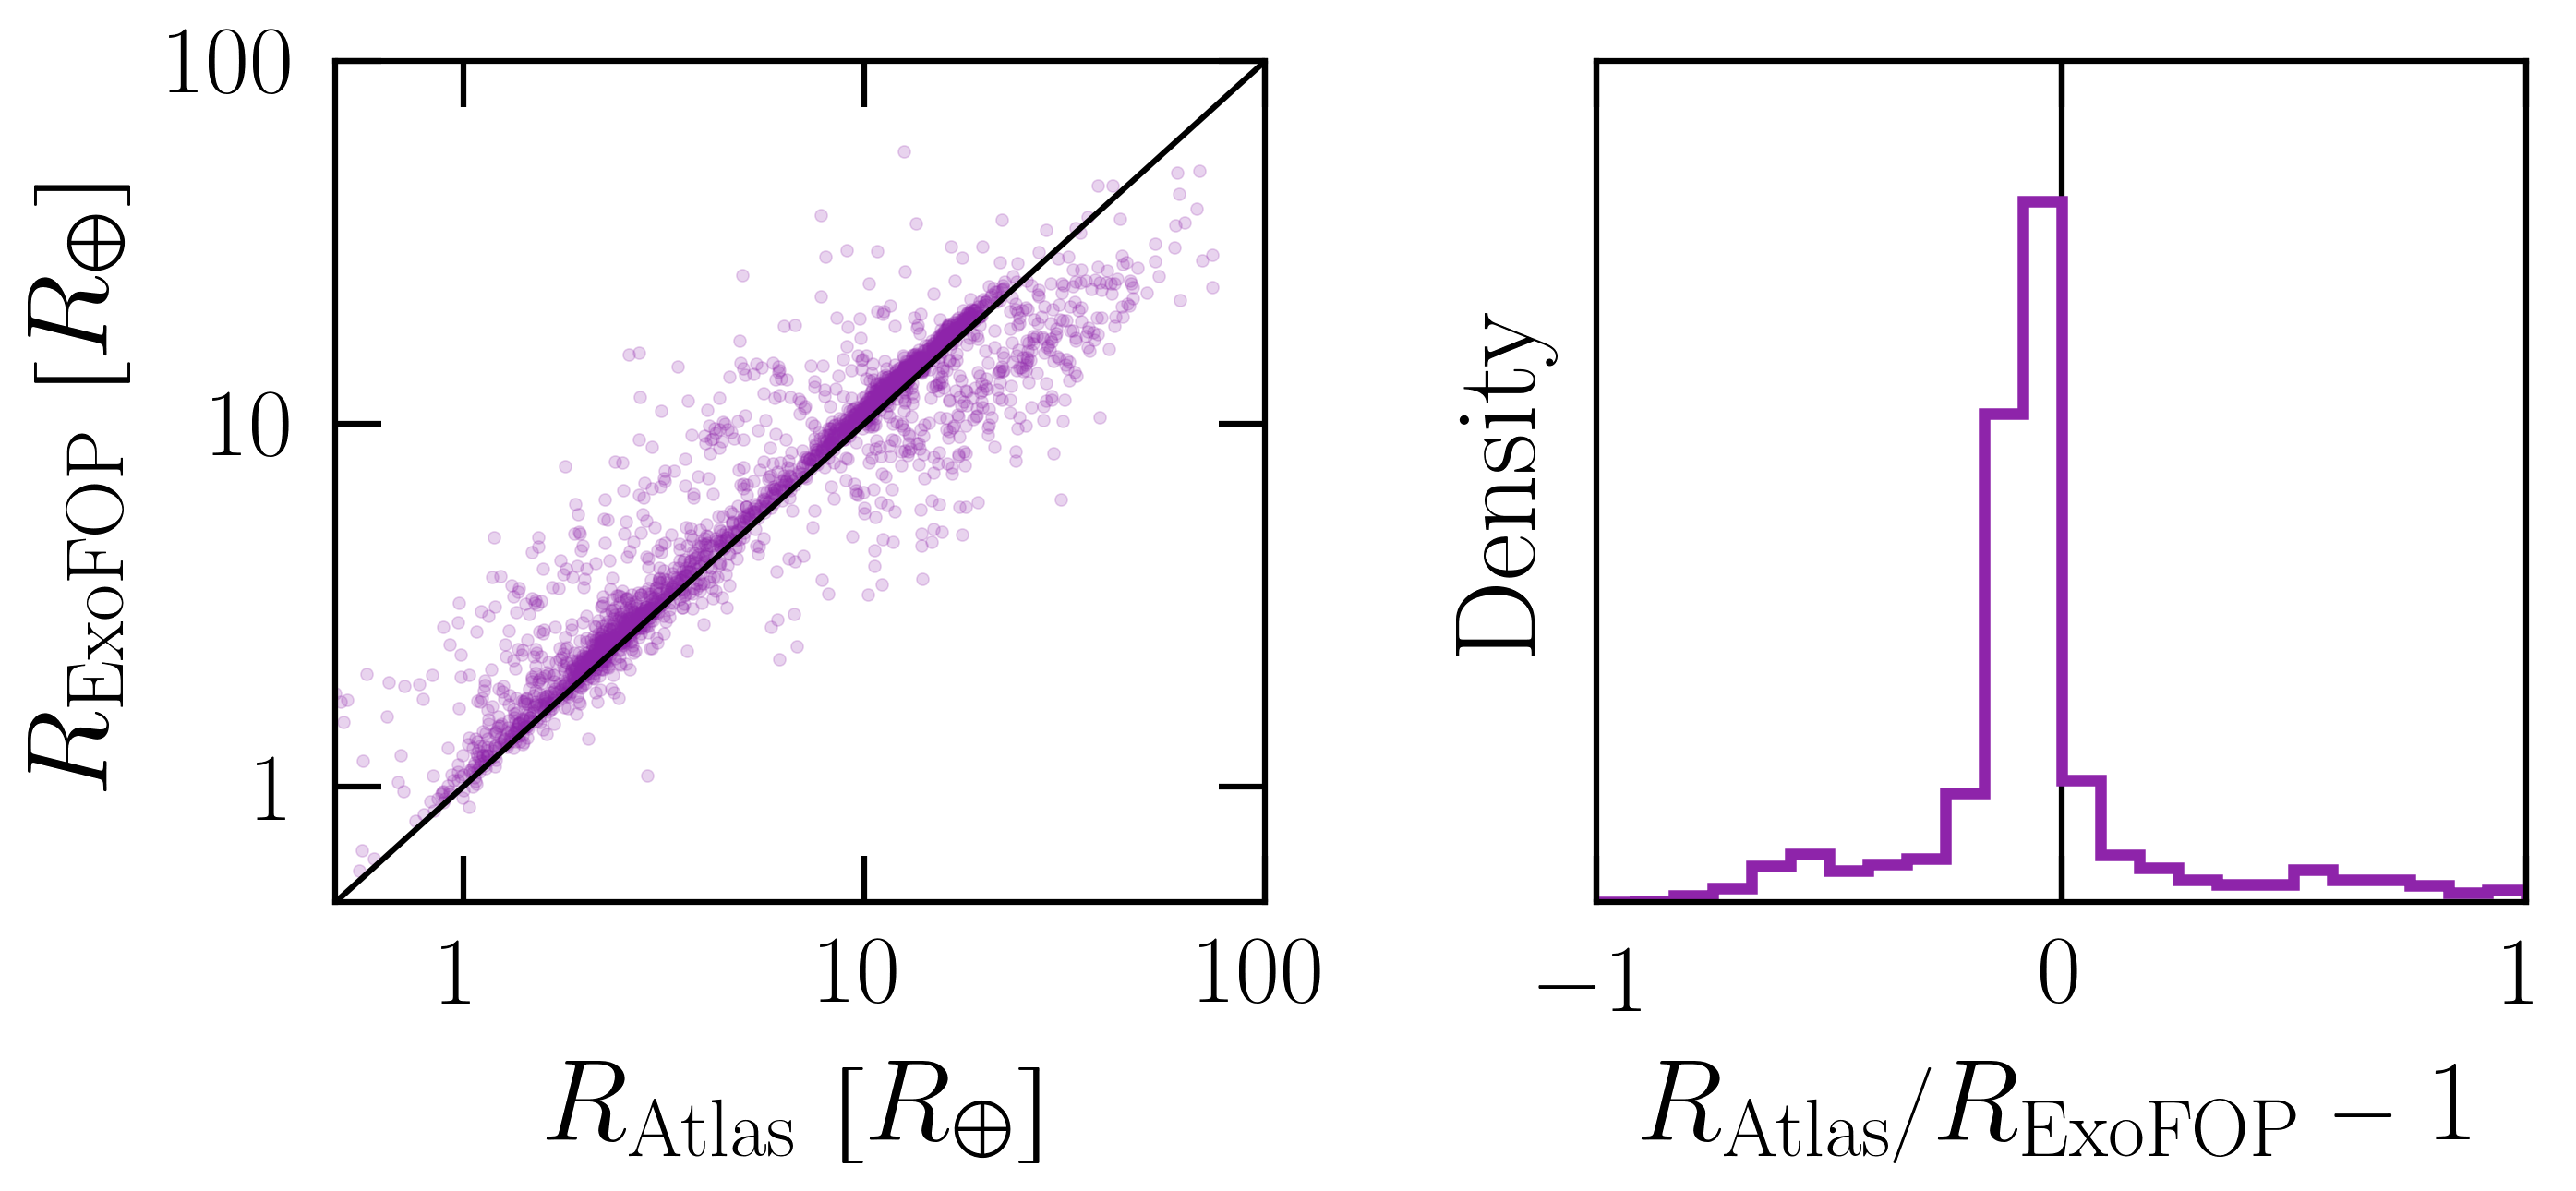
\includegraphics[width=\linewidth]{figures/radius_error.png}
  \caption{\textbf{Comparing :} . The black line shows the one- to-one correspondence. As expected, there is good agreement between the two methods although the MCMC values are systematically smaller than those found by DV. The largest disagreement is typically for KOIs with large fit values for impact parameter. }
  \label{fig:}
\end{figure}





\section{Discussion}\label{sec:conclusion}
We present for the first time a catalog of Bayesian posterior samples for the 2-minute cadence TOIs from 2018-2022.
Some words about results.
Some stuff about difficulty sampling grazing systems.
Errors when SPOC estimates are off.
We expect the remainder of the \tess\ extended mission will complete by September 2023, at which point an updated catalog will be produced.

Vetters can identify false positive TCEs by a few tell- tale signs: a visible secondary eclipse which cannot phys- ically be planetary in nature; a mismatch between odd and even transit depths caused by a stellar binary at twice the indicated period; a shift of the centroid to another nearby star; and increasing transit depth with aperture size, indicative that a signal is from an object nearby on the sky and not the suspected target star.

Lots of manual vetting requiured to promote TCE to TOI. In the future this work can help with that process.


Although in practice most applications will use the best available stellar characterization to place at least a modestly in- formative prior on rho star (and, indirectly, on T and e via the photoeccentric effect), for our present experiment we are more concerned with the sampler behavior (i.e. whether MCMC chains are well behaved) rather than the poste- rior inferences.

We should use the grazing transit umbrella method 


\section{Data and software availability}\label{sec:data}
Software to carry out this analysis on github.

Data for analysis obtained from exofop, MAST. 

Our analysis data products are availible on the website.

Can be downloaded from the website.

Alternatively, if a user installs the `tess-atlas` python package, they can use the command line interface to download the data and notebooks.

download toi to get one analysis
download population summary
download all fits


Demo both python interface to load stuff andd the CLI interface to download stuff.

%%%%%%%%%%%%%%%%%%%%



\section*{Acknowledgments}{

We would like to thank xyz.
Ozgrav, Flatiron, NECTAR, ADACS, David Liptai
Work was started during `online.tess.science`

This work has used the TIC through the TESS Science Office’s target selection working group (architects K. Stassun, J. Pepper, N. De Lee, M. Paegert, R. Oelkers).

This research has made use of the NASA Exoplanet Archive, which is operated by the California Institute of Technology, under contract with the National Aeronautics and Space Administration under the Exoplanet Exploration Program.

This work made use of the \tess\ catalog on ExoFOP

Total compute time for this work \red{\cpuHrs} \alltodo{get more accurate compute time (this is an overestimate)}. CO$_2$ emission amount for this work would be XX, however as OzStar uses wind energy this has a negligible carbon footprint.

}

\vspace{5mm}
\facilities{\tess, \gaia, \kepler, Exoplanet Archive, etc.}

\software{
astropy~\citep{Astropy-Collaboration:2013,Astropy-Collaboration:2018},
exoplanet,
lightkurve,
starry,
celerite2,
pymc3~\cite{Salvatier:2016:ascl},
numpy,
scipy,
pandas,
matplotlib,
corner,
sphinx,
}


% ADS bibliography link
% https://ui.adsabs.harvard.edu/user/libraries/_DyLS4HbTY-eJIMBiFUdxw
\bibliography{atlas}{}
\bibliographystyle{aasjournal}

%%%%%%%%%%%%%%%%%%%%%%%%%%%%%%%%%%%%%%%%%%%%
\appendix

\section{Computing the implied stellar density}\label{apdx:stellar_density}
For a circular orbit, the transit duration is \citep{Winn:2010:arXiv}
\begin{equation}~\label{eq:tau}
  \tau = \frac{P}{\pi}\,\sin^{-1}\left( \frac{\sqrt{(1 + (R_{p}/R_{\star})^2) - b^2}}{a\,\sin i} \right) \quad. \,
\end{equation}
where $a$ is the semi-major axis in units of $R_\star$. 
Rearranging Eq~\ref{eq:tau} in terms of $a$, we find that
\begin{equation}~\label{eq:a1}
  a^2\,\sin^2 i\,\sin^2\left(\frac{\pi\,\tau}{P}\right) = (1 + (R_{p}/R_{\star})^2) - b^2 \quad.
\end{equation}
Since $\cos^2 i = b^2 / a^2$, Eq~\ref{eq:a1} can be simplified
\begin{equation}
  a^2 = \frac{(1 + R_{p}/R_{\star})^2 - b^2\,\cos^2\phi}{\sin^2\phi}
\end{equation}
for $\phi = \pi\,\tau / P$.

Finally, under the assumption of a circular orbit, we can compute the implied stellar density $\rho_\mathrm{circ}$ with the period and semi-major axis
\begin{equation}
  \rho_\mathrm{circ} = \frac{3\,\pi\,a^3}{G\,P^2} \quad.
\end{equation}



\end{document}
